\documentclass[xcolor=pdftex,dvipsnames,table,mathserif,aspectratio=169]{beamer}
\usetheme{metropolis}
%\usetheme{Darmstadt}
%\usepackage{times}
%\usefonttheme{structurebold}

\usepackage[english]{babel}
%\usepackage[table]{xcolor}
\usepackage{pgf,pgfarrows,pgfnodes,pgfautomata,pgfheaps}
\usepackage{amsmath,amssymb,setspace,centernot}
\usepackage[latin1]{inputenc}
\usepackage[T1]{fontenc}
\usepackage{relsize}
\usepackage{pdfpages}
\usepackage[absolute,overlay]{textpos} 

\DeclareMathSizes{10}{10}{6}{6} 


\title [Dynamic Demand I]{Dynamic Demand I:\\
 Overview}
\author{C.Conlon}
\institute{Grad IO}
\date{\today}
\setbeamerfont{equation}{size=\tiny}
\begin{document}

\begin{frame}
\titlepage
\end{frame}


\begin{frame}{Dynamic Demand}
\begin{itemize}
\item Earlier this term we looked at \textit{static models of product differentiation} such as BLP (1995).
\item We have also looked at single agent models of dynamic behavior such as Rust (1987).
\item What if we could put those two together? Why?
\end{itemize}
\end{frame}

\begin{frame}{Dynamic Demand}
What about the following questions?
\begin{itemize}
\item Secondary Markets: Good or bad for sellers? overall welfare?
\begin{itemize}
\item I may pay \alert{more} for a new car today because I can sell it tomorrow.
\item I may pay \alert{less} for a new car today because of competition with used cars.
\end{itemize}
\item Durability: Should products be built to last longer or shorter?
\begin{itemize}
\item I pay \alert{more} for an appliance (dishwasher, car, microwave, IPhone, Computer, etc.) if it 
\alert{lasts longer}.
\item But, I will re-purchase less frequently (Maytag Repairman)
\end{itemize}
\end{itemize}
\end{frame}


\begin{frame}{Dynamic Demand}
What about the following questions?
\begin{itemize}
\item Adoption or Scrappage Subsidies
\begin{itemize}
\item Cash-For-Clunkers paid a rebate to replace your old car (Explorer/Caravan) with a new fuel-efficient one (Corolla)
\item Was this about being green or about bailing out auto industry?
\end{itemize}
\item Temporary Sales: Why do some products have them?
\begin{itemize}
\item Pure price discrimination (attracting low-value buyers?) 
\item Attracting switchers/ state dependence?
\item Intertemporal price discrimination with storage?
\end{itemize}
\end{itemize}
\end{frame}



\begin{frame}{Dynamic Demand}
Thus far we have implicitly assumed you buy a product and you receive all utility from consumption immediately. We could think about each period receiving a \alert{flow payment} $f_{ijt}$. However, most of the time we could just write the NPV of future discounted flow payoffs as a \alert{lump sum}:
\begin{align*}
v_{ijt} = \sum_{t=0}^{\infty} \beta^t \cdot f_{ijt}
\end{align*}
and compare lump sum / NPV payoffs: $v_{ijt}$ vs $p_{jt}$ for different goods.
\begin{itemize}
\item For things like yogurt --we probably don't need to model when you choose to consume the yogurt separately from purchase.
\item Maybe the good depreciates over time $f_{ijt} \geq f_{ij,t+1}$ (fine).
\item Maybe it breaks with some probability $\rho_t$ (in which case I could use ``expected NPV'').
\item But...
\end{itemize}
\end{frame}



\begin{frame}{Rentals?}
Another way to think about dynamics is to think about the rental rate:
\begin{itemize}
\item A house or car or other durable has a per-period price
\begin{align*}
\Delta p_{j,t}=p_{j,t+1} - p_{j,t}
\end{align*}
\item You buy it and pay $p_{j,t}$ and sell it to the market at $p_{j,t+1}$ each period.
\item Each period you ``rent'' the product to yourself at $\Delta p_{j,t}$.
\item This only makes sense if the secondary market is frictionless (or we have to include a ``switching'' term)
\begin{itemize}
	\item Gavazza, Lizzeri, Roketskiy (AER 2014) do this for cars.
	\item Kalouptsidi (AER 2014) does this to pin down the value function.
\end{itemize}
\end{itemize}
\end{frame}



\begin{frame}{CPI: High Tech Durables}
\begin{figure}[htbp]
\begin{center}
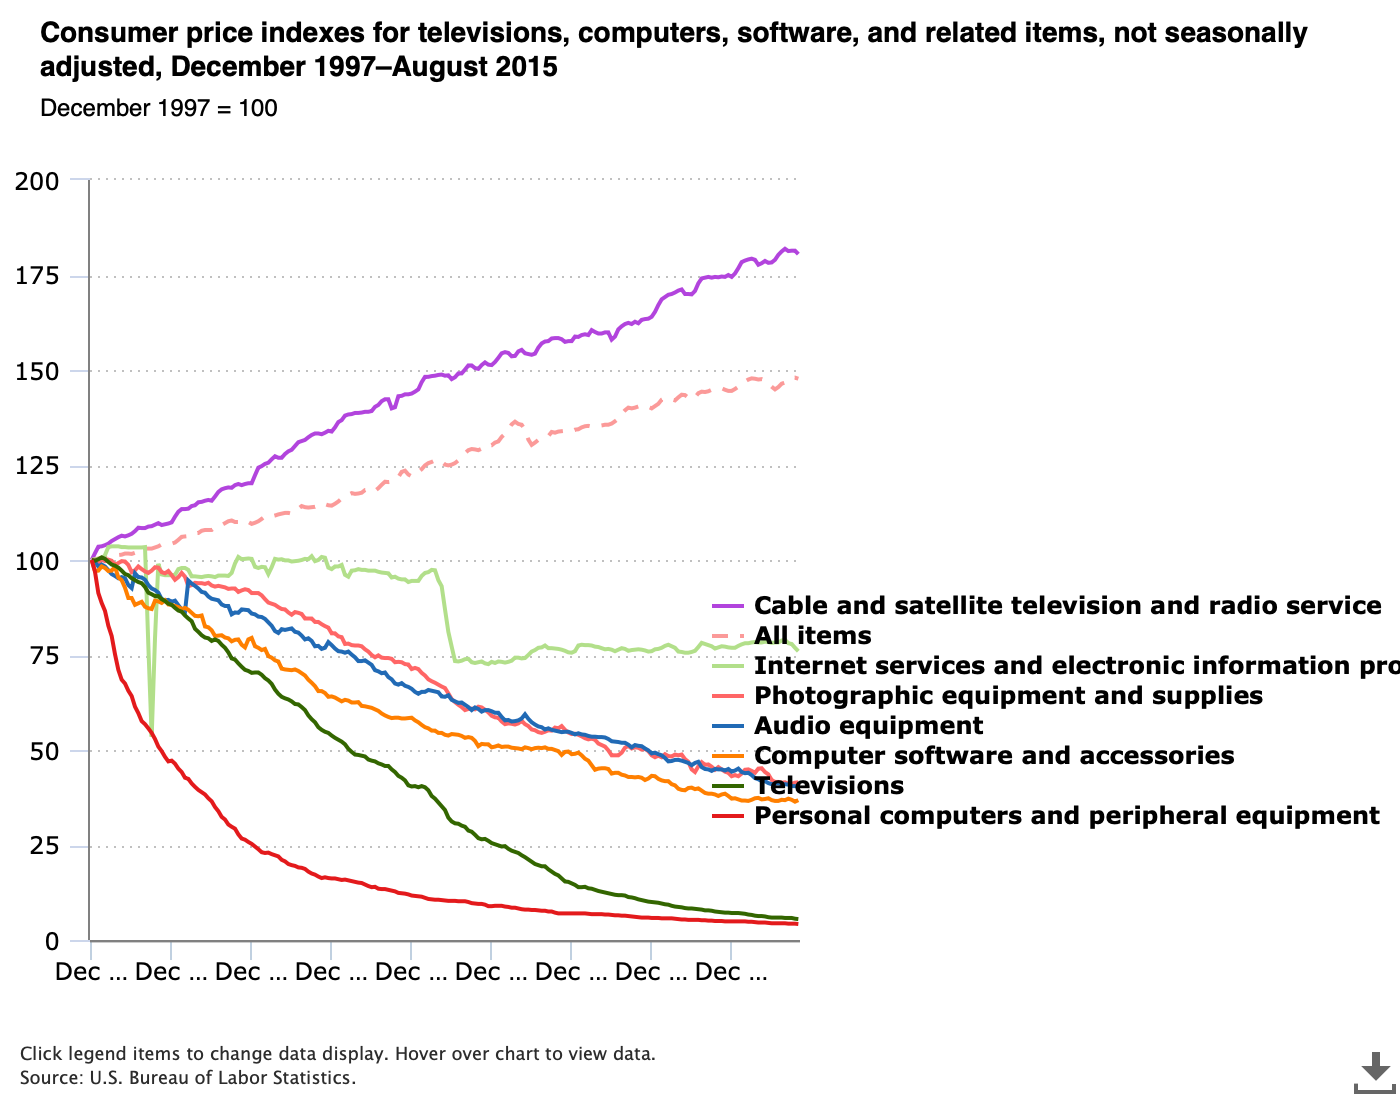
\includegraphics[width=3.75in]{resources/cpi_chart.png}
\label{gandr2}
\end{center}
\end{figure}
\end{frame}


\begin{frame}{High Tech Durables}
\begin{itemize}
\item Today a 55" 4K LCD TV is \$239. In 2006, you could buy a 32" 720P TV for $>\$10,000$.
\item In December 2011 TV prices fell $17\%$ on an annual basis and other A/V equipment fell $11\%$, and computer equipment fell $14\%$.
%\item Conlon 2016 reports a 22\% annualized price decline in LCD TV's from 2006-2009.
\item From August 2005 to August 2015 prices declined by 87.2\%.
\item We might also find that over time consumers buy better cameras or larger TV's
\item The BLS tries to do \textit{chaining} and \textit{quality adjustments} but in high-tech products this can be very difficult.
\item This has a potentially large impact on price indices (a small bias in the CPI can be billions of dollars in SSA/Medicare payments).
\end{itemize}
\end{frame}


\begin{frame}{Adoption Curve}
\begin{figure}[htbp]
\begin{center}
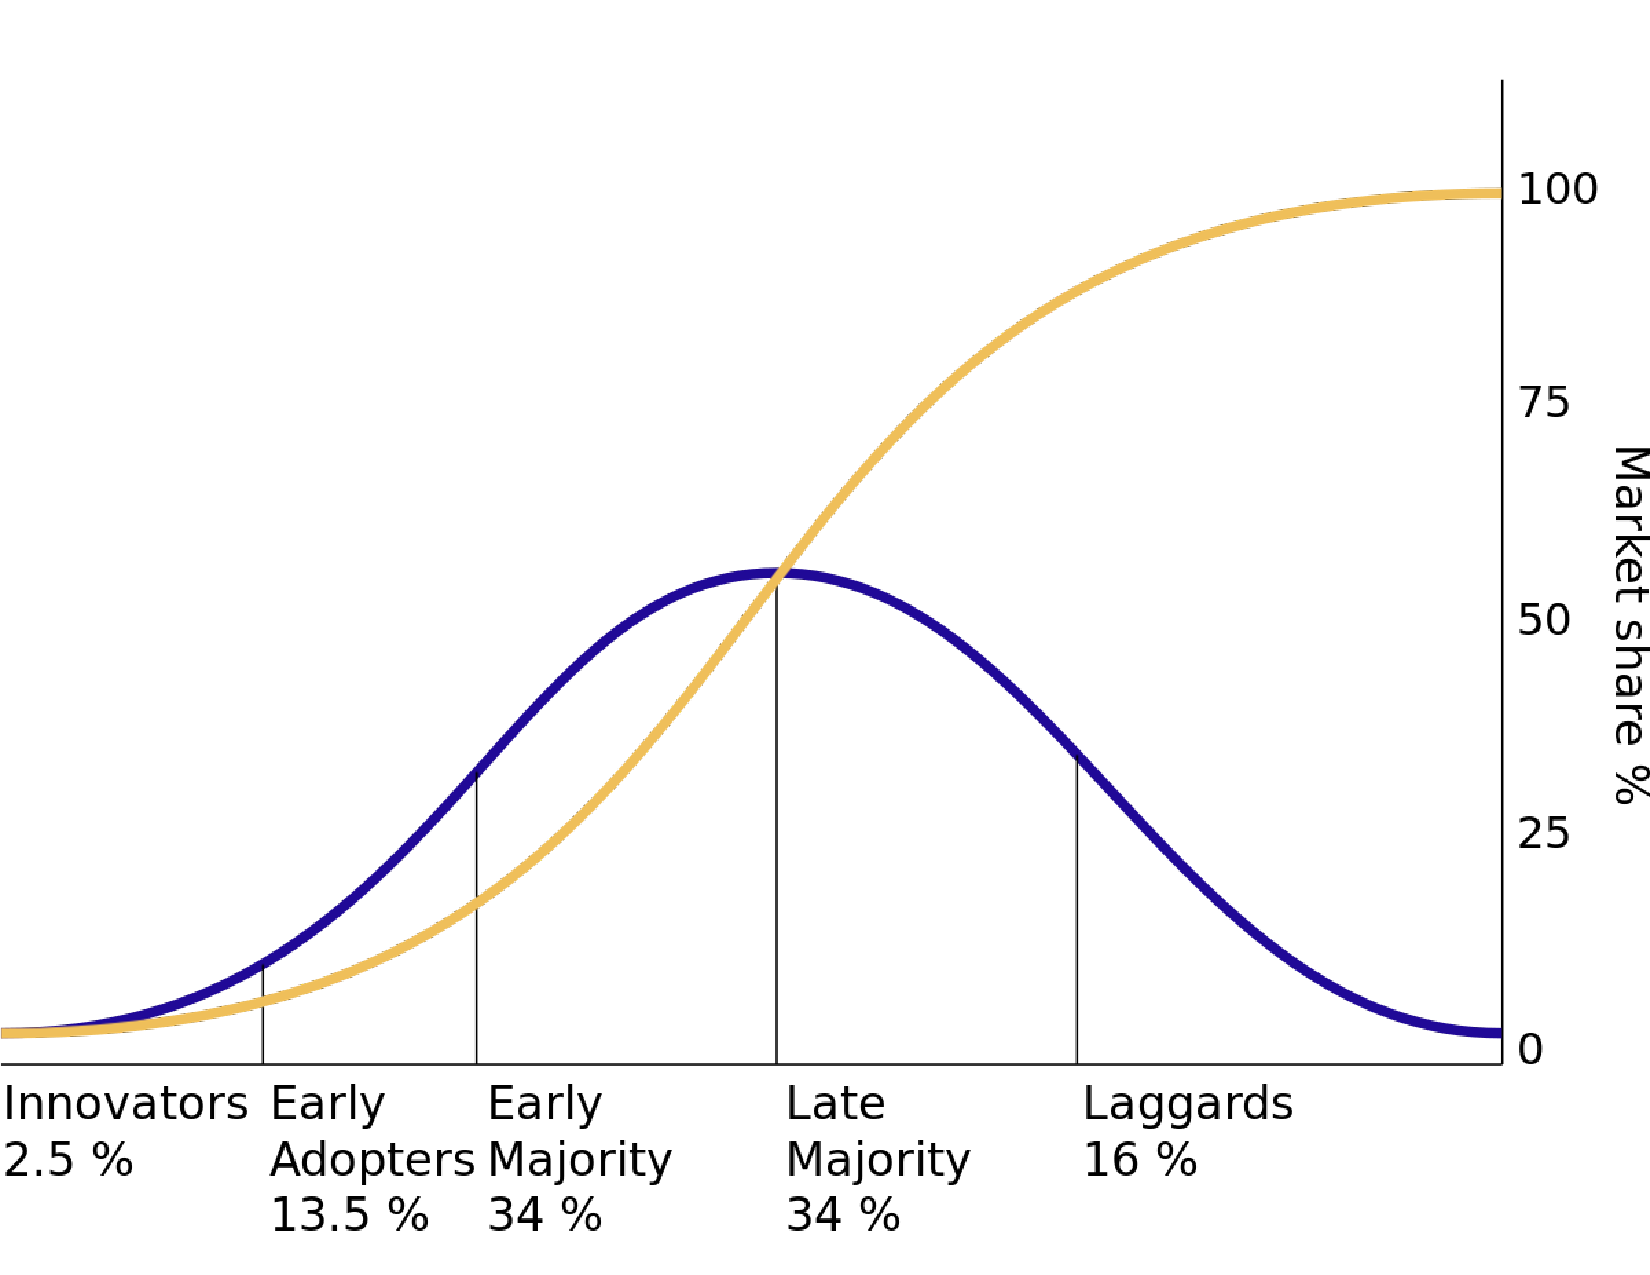
\includegraphics[width=3.75in]{resources/s_curve.pdf}
\label{gandr2}
\end{center}
\end{figure}
\end{frame}

\begin{frame}{Dynamic Demand  (Gowrisankaran Rysman)}
\begin{figure}[htbp]
\begin{center}
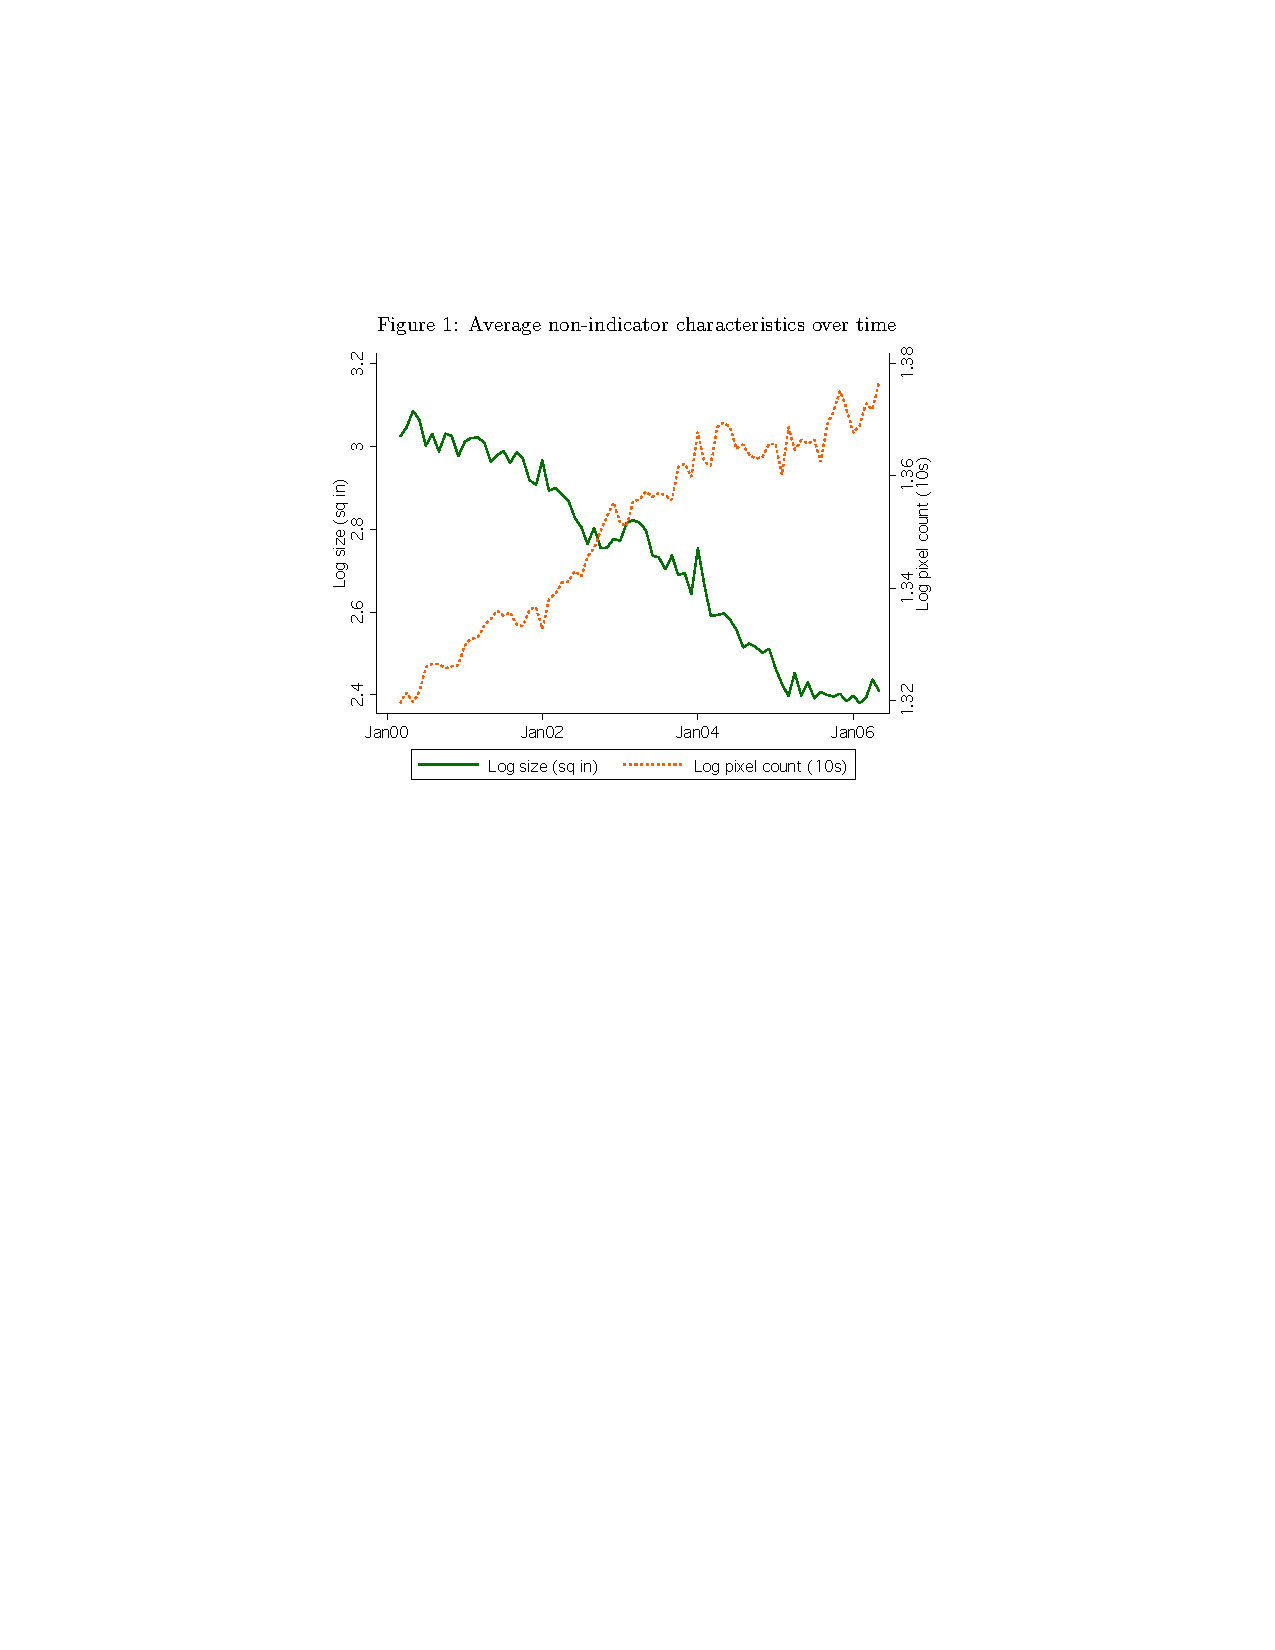
\includegraphics[width=4in]{resources/gandr1.pdf}
\label{gandr1}
\end{center}
\end{figure}
\end{frame}

\begin{frame}{Dynamic Demand (Gowrisankaran Rysman)}
\begin{figure}[htbp]
\begin{center}
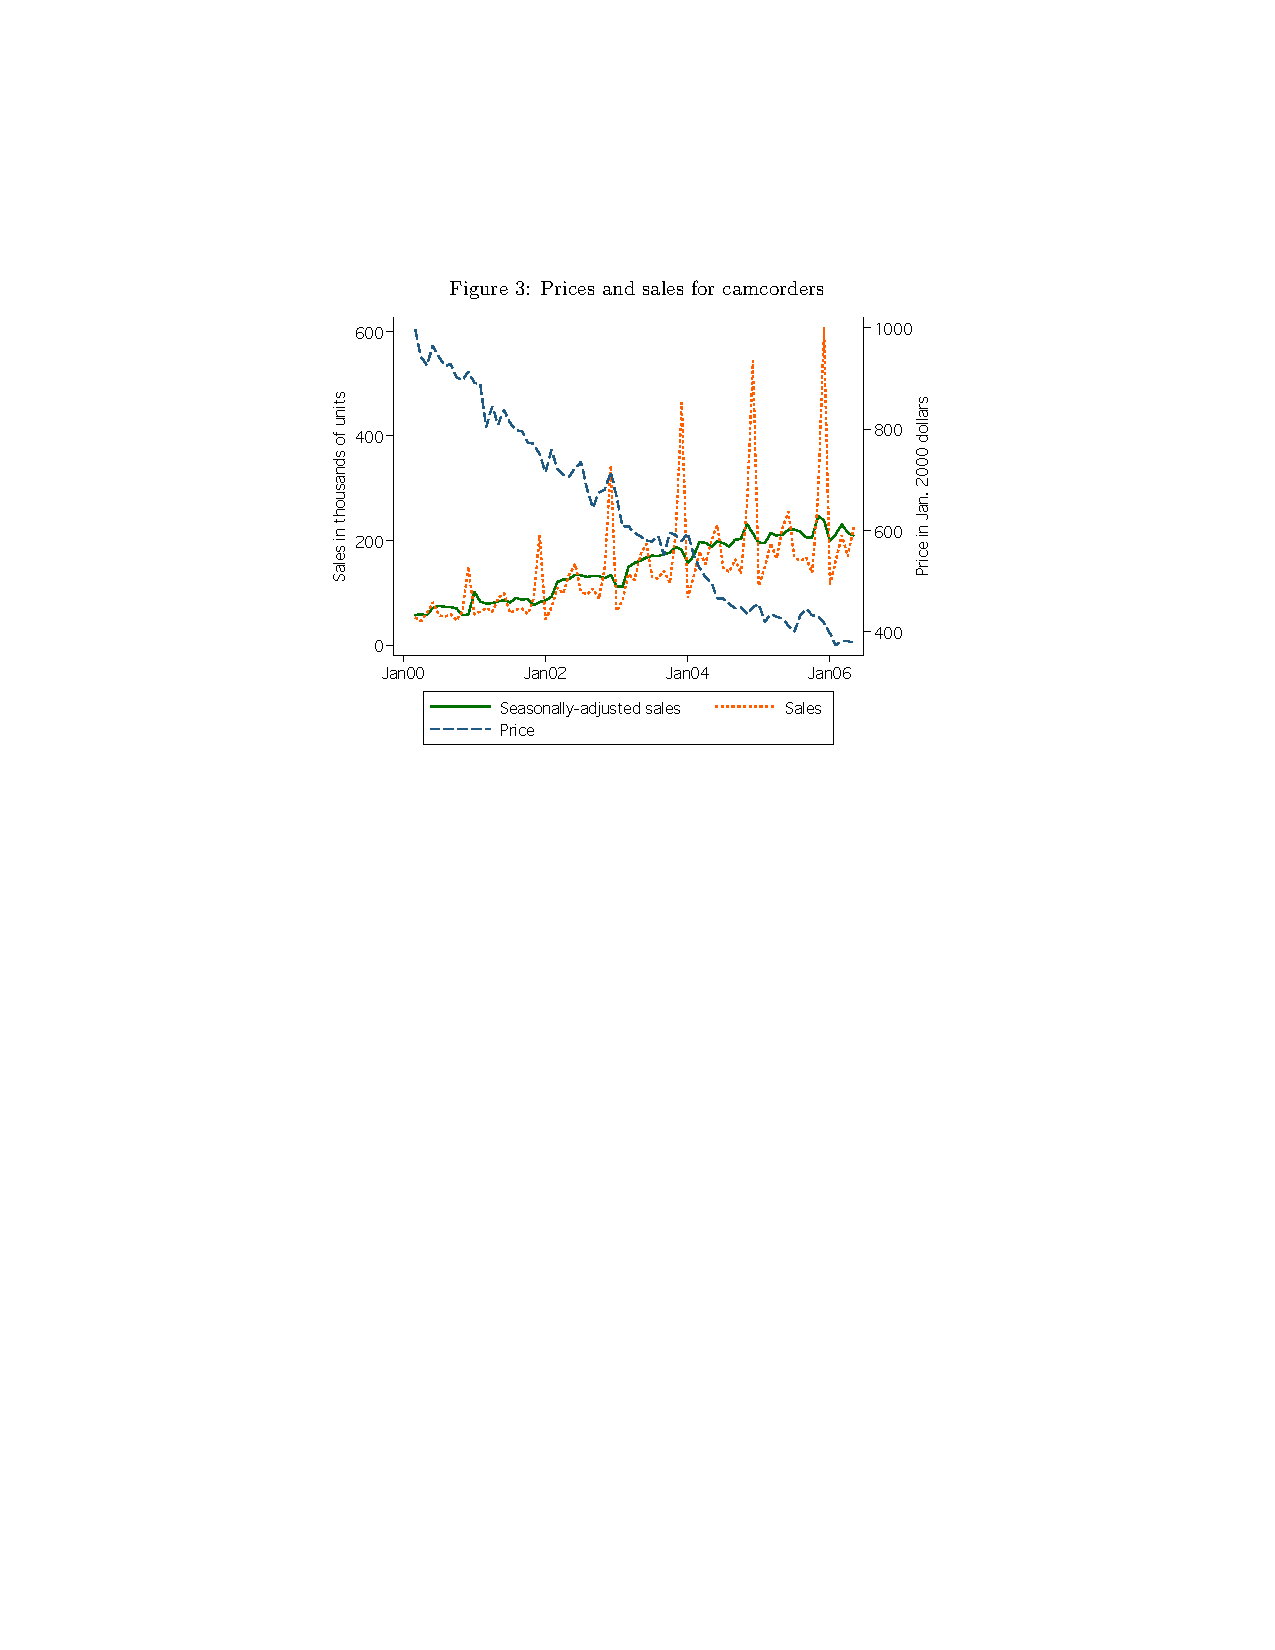
\includegraphics[width=4in]{resources/gandr2.pdf}
\label{gandr2}
\end{center}
\end{figure}
\end{frame}

\begin{frame}{High-Tech Durables}
Imagine if we regressed $P$ on $Q$ (with the usual static IV):
\begin{itemize}
\item In early periods $P$ falls and $Q$ rises.
\item In later periods $P$ falls and $Q$ also falls (top of the $S$-curve).
\item Depending on the time period we might find that demand slopes \alert{upwards} (lower prices lead to lower sales)
\end{itemize}
\end{frame}

\begin{frame}{Dynamic Demand: Infeasible Static Approach}
Think about this model:
\begin{align*}
u_{ijt} &=   \alpha_i x_{jt}  +  \xi_{jt} + \varepsilon_{ijt}\\
u_{i0t} &=  \alert{\overline{u}_{i0t}} + \varepsilon_{i0t} 
\end{align*}
\vspace{-0.5cm}
\begin{itemize}
\item The real problem is that $\overline{u}_{i0t}=0$ for all $(i,t)$ is a bad assumption.
\item If we knew $\overline{u}_{i0t}$, we could plug it in, estimate a static model and be fine.
\item $\overline{u}_{i0t}$ includes several things:
\begin{itemize}
	\item How good is my current TV/Camera/Car today? $f_{i0t}$. (Initial conditions may differ)
	\item What will happen tomorrow / what do I anticipate (new IPhone debut, price cuts for Black Friday, etc.)
\end{itemize}
\item \alert{Idea: use the realization of $t+1$ to inform outside option today (Rust!)}
\end{itemize}
\end{frame}

\begin{frame}{Ad-Hoc approach}
\begin{itemize}
\item  Just proxy with a time trend or sieve (Lou Prentice Ying 2012), (Eizenberg 2011) etc.  That is $u_{i0t} = \gamma_{0i} + \gamma_{1i} t + \gamma_{2i} t^2 + \ldots$
\item We can get the elasticity correct.
\item Not structural! Not helpful if we want to do counterfactuals! Can't get the elasticities under different conditions.
\item Is $u_{i0t}$ about current durable value? or Equilibrium beliefs about the future? (both!)
\item Do we have $i$ specific coefficients (we should!)
\end{itemize}
\end{frame}
% \begin{frame}{Two Examples}
% \begin{itemize}
% \item High Tech Durables
% \begin{itemize}
% \item We are often interested in the case where a firms' products compete not only against products of other firms, but also with their own products over time. (Coase 1972).
% \item Really this is a feature of any kind of durable (cars, washing machines, etc.).
% \item In high-tech products, we have `S'-shaped penetration curve. At some point we cut the prices of (computers, cameras, TV's) and the sales go down rather than up. Why?
% \item Static estimates imply demand is \alert{less elastic} than it really is.
% \end{itemize}
% \item Storable Goods
% \begin{itemize}
% \item Laundry detergent goes on discount: $\approx$ 1 week in every 4-8.
% \item A large fraction of overall quantity is sold during these discount weeks.
% \item This would imply highly elastic demand. (1) Laundry detergent business must be extremely competitive. (2) There would be a substantial response to a \alert{permanent} price change. Seems unlikely that (1) and (2) are true.
% \item Static estimates imply demand is \alert{more elastic} than it really is.
% \end{itemize}
% \end{itemize}
% \end{frame}

%\begin{frame}{Dynamic Demand}
%\begin{figure}[htbp]
%\begin{center}
%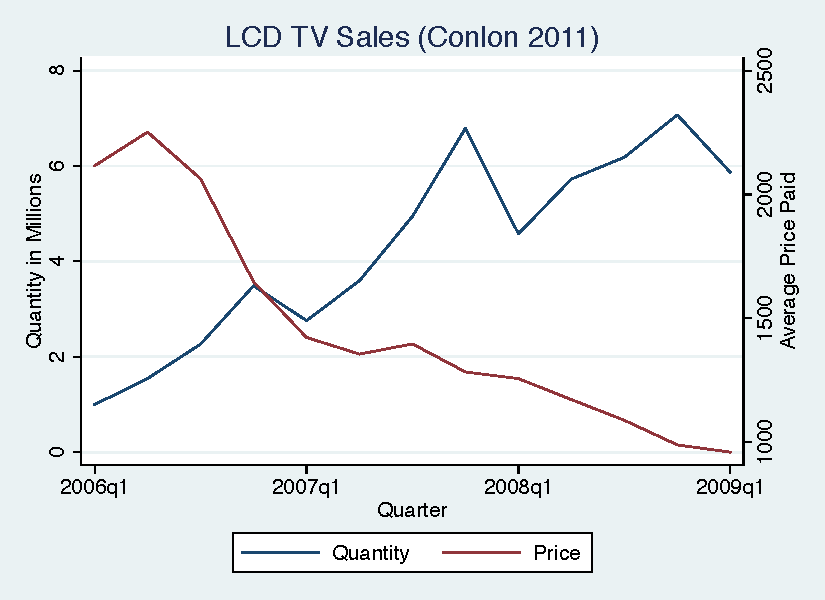
\includegraphics[width=4in]{resources/conlon1.pdf}
%\label{conlon1}
%\end{center}
%\end{figure}
%\end{frame}
%
%\begin{frame}{Dynamic Demand}
%\begin{figure}[htbp]
%\begin{center}
%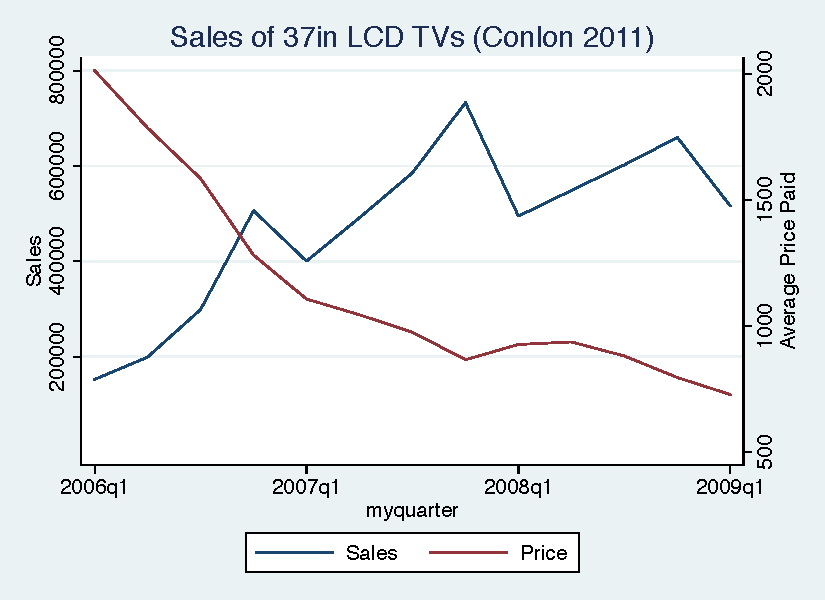
\includegraphics[width=4in]{resources/conlon2.pdf}
%\label{conlon1}
%\end{center}
%\end{figure}
%\end{frame}




\begin{frame}{Dynamic Demand: Stripped Down Version}
Let's start with some very strong assumptions to get our intuition clear:
\begin{enumerate}
\item There are $t=1,2$ periods.
\item Consumers can purchase at most one unit of an (infinitely) durable good
\item After purchasing the durable good they leave the market forever.
\end{enumerate}
\end{frame}

\begin{frame}{Dynamic Demand: Naive Static Approach}
\begin{align*}
u_{ijt} &=   \alpha_i x_{jt}  +  \xi_{jt} + \varepsilon_{ijt}\\
u_{i0t} &=  \varepsilon_{i0t} 
\end{align*}
\begin{itemize}
\item Suppose  we estimate demand treating each period $t=1,2$ as a \alert{separate market}.
\item ie: close our eyes and do BLP.
\item What do we get wrong?
\begin{itemize}
\item How does $\frac{\partial q_{j,t}}{\partial p_{k,s}}$ look? How should it look?
\end{itemize}
\item Three problems: 
\begin{itemize}
\item period $t=1$ and $t=2$ are \alert{substitutes}
\item distribution of $f(\alpha_{it})$ is likely different in $t=1,2$.
\item Is $E[u_{i0t}]$ the same for all $(i,t)$?
\end{itemize}
\end{itemize}
\end{frame}




\begin{frame}{Dynamic Demand: Complete Information}
Suppose consumers have full information about all shocks $(x_{j1},x_{j2},\xi_{j1},\xi_{j2},\varepsilon_{ij1},\varepsilon_{ij2})$ in both periods. 
\begin{align*}
u_{ijt} &=   \alpha_i x_{jt}  +  \xi_{jt} + \varepsilon_{ijt}
\end{align*}
What would we do?
\begin{itemize}
\item Why not estimate static demand among $\bigcup_{t=1,2}  \mathcal{J}_t $ alternatives?
\item Remaining issues:
\begin{itemize}
\item Buying in period 1 allows me an additional period of consumption
\item Need to discount period 2 utility $\beta \times ( \alpha_i x_{jt}  +  \xi_{jt} + \varepsilon_{ijt})$ or $\beta \times ( \alpha_i x_{jt}  +  \xi_{jt} )+\varepsilon_{ijt}$
\item A single outside good of not purchasing in either period $ u_{i0} =  \varepsilon_{i0} $
\end{itemize}
\item How bad is this model? Compared to the last one?
\end{itemize}
\end{frame}



\begin{frame}{Dynamic Demand: Relaxing some assumptions}
Problematic assumption was probably full information. Suppose instead that only $(\varepsilon_{ij2},\varepsilon_{i0})$ are \alert{unobserved} in $t=1$. 
\begin{align*}
v_{i0,t=1} \equiv E_{\varepsilon} [\max_j u_{ij2} | \Omega_{t=1} ] = \log \left( \sum_j \exp [ \alpha_i x_{j2}  +  \xi_{j2} ] \right) + \eta
\end{align*}
\begin{itemize}
\item $\Omega_{t=1}= \{x_{j1},x_{j2},\xi_{j1},\xi_{j2},\varepsilon_{ij1}\}$ (everything known at $t=1$) 
\item $\eta$ is Euler's constant (per usual).
\item What about outside good?
\begin{itemize}
\item Either just another good in $t=2$ with $\alpha_i x_{j2}+ \xi_{j2} = 0$
\item Or we consider $v_{i0,t=2}=E [\max \{ \varepsilon_{i0}, \max_j u_{ij2} \}  | \Omega_{t=1}]$
\end{itemize}
\end{itemize}
\end{frame}

\begin{frame}{Dynamic Demand: What about Beliefs?}
\begin{itemize}
\item This assumed that $x_{j2}$ and $\xi_{j2}$ were observed in $\Omega_{t=1}$.
\item Maybe we want to make some component of $x_{j2}$ \alert{unobserved} (such as price or $\xi$).
$$
E_t\left[ \log \left( \sum_j \exp [ \alpha_i p_{j2}  +  \xi_{j2} ] \right)\big| \Omega_t\right]= 
\int \log \left( \sum_j \exp [ \alpha_i p_{j2}  +  \xi_{j2} ] \right)  g(\mathbf{p_2} | \Omega_t) 
$$
\end{itemize}
Integrate out over the unknown (distribution depends on information $\Omega_t$)
\end{frame}

\begin{frame}{Dynamic Demand: Rational Expectations}
$$
E_t\left[ \log \left( \sum_j \exp [ \alpha_i x_{j2}  +  \xi_{j2} ] \right)\big| \Omega_t\right]= 
\log \left( \sum_j \exp [ \alpha_i x_{j2}  +  \xi_{j2} ] \right)  + \eta+  \zeta_{it}
$$
Rational expectations implies that expectational error $\zeta_{it}$ is orthogonal to everything known at $\Omega_t$
\begin{itemize}
\item Can't use anything in $\Omega_t$ to predict $\zeta_{it}$ so $E_t[\zeta_{it} \times A(\Omega_t)]=0$
\end{itemize}
\end{frame}

\begin{frame}{Dynamic Demand: Relaxing some assumptions}
Now what?
\begin{align*}
u_{ij,t=1} &=   \alpha_i x_{j1}  +  \xi_{j1} + \varepsilon_{ij1}\\
u_{i0,t=1} &=  \overline{u}_{i0,t=1}+  \alert{\beta v_{i0,t=1}} + \zeta_{i,t=1}+ \varepsilon_{i01} \\
u_{ij,t=2} &=   \alpha_i x_{j2}  +  \xi_{j2} + \varepsilon_{ij2}\\
u_{i0,t=2} &= \overline{u}_{i0,t=2} +  \alert{\underbrace{\beta v_{i0,t=2}+ \zeta_{i,t=2} }_{=0}}+\varepsilon_{i02} 
\end{align*}
\vspace{-.5cm}
\begin{itemize}
\item If $(\overline{u}_{i0,t}, \beta v_{i0,t=1})$ are known we can estimate static demand with each $t$ as a separate ``market''.
\item I pulled an extra $\varepsilon_{i01}$ out of my hat.
\item What is the other dynamic linkage?
\end{itemize}
\end{frame}


\begin{frame}{Dynamic Demand: What about cream skimming?}
Also need to account for the fact that $f(\alpha_{i,t=1})$ and $f(\alpha_{i,t=2})$  are not the same:
\begin{itemize}
\item If goods are perfectly durable, and consumers permanently exit the market...
\item Assume that $f(\alpha_{i,t=1}) = w_{i,t=1}$ is a discrete distribution of ``types''
\begin{itemize}
\item Note: ``type'' does not include $\varepsilon$.
\item then $w_{i,t=2} = w_{i,t=1} \cdot s_{i0,t=1}$
\end{itemize}
\end{itemize}
\end{frame}




\begin{frame}{Dynamic Demand: Can we go further?}
Replacement / Upgrades:
\begin{itemize}
\item Suppose we allow the people who purchase in $t=1$ to remain in the market.
\item Now part of your ``type'' $\alpha_i$ includes your existing stock of the durable good $\overline{u}_{i0t}$
\begin{itemize}
\item Think about as a RC on the constant $\beta_{i0}$
\end{itemize}
\item A purchase increases the value of outside good (previously to $\infty$)
\item The transitions become more complicated $w_{t=2} = f(w_{t=1},s_{ij,t=1})$.
\begin{itemize}
\item You still throw the old durable into the trash when you are done.
\begin{itemize}
\item Could also allow for a scrap value.
\end{itemize}
\item Need to be a bit careful about NPV of expected stream of payments vs. ``flow utility'' now.
\end{itemize}
\end{itemize}
\end{frame}


\begin{frame}{Dynamic Demand: Storable Goods}
\begin{itemize}
\item Same idea:
\begin{align*}
u_{ijt} &=   \alpha_i x_{jt}  +  \xi_{jt} + \varepsilon_{ijt}\\
u_{i0t} &=  \alert{\overline{u}_{i0t}} + E[\max_j u_{ij,t+1}| \Omega_t] + \varepsilon_{i0t} 
\end{align*}
\item My type $\overline{u}_{i0t}$: how much laundry detergent I have left.

\item My beliefs $E[\max_j u_{ij,t+1}| \Omega_t]$: is my preferred brand likely to be on discount in the near future?
\item Bias from $u_{i0t} = \varepsilon_{i0t}$. Sales are high during discounts and low following discounts. We think this implies demand is \alert{too elastic} relative to a permanent price change.
\item Durables $Corr(u_{i0t},p_{jt}) <0$ (time trend).\\
 Storables: $Corr(u_{i0t},p_{jt}) > 0 $ (sale in adjacent period).
\end{itemize}
\end{frame}


\end{document}













































